% Figures for the GF180MCU multi-block SoC (v3). pdfLaTeX, IEEEtran.
% Requires \usepackage{graphicx}. Place the PDF files next to the .tex file.

\begin{figure*}[!t]
\centering
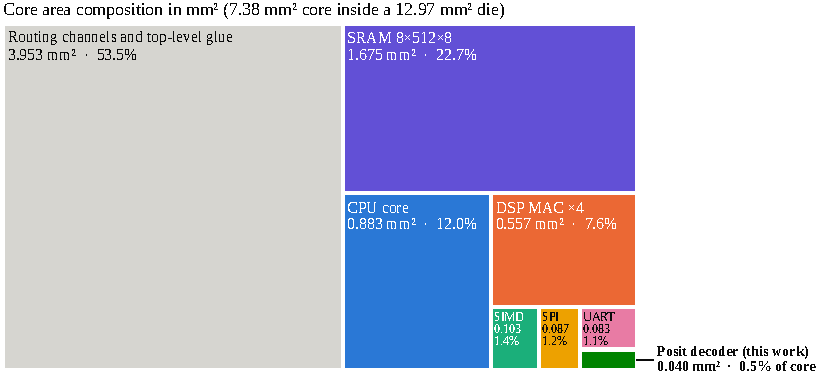
\includegraphics[width=\textwidth]{fig01_area_treemap.pdf}
\caption{Core area composition of the SoC. The routing channels hold the top-level glue logic and repeaters. The proposed posit decoder occupies 0.040\,mm$^2$, or 0.5\% of the core.}
\label{fig:area}
\end{figure*}

\begin{figure}[!t]
\centering
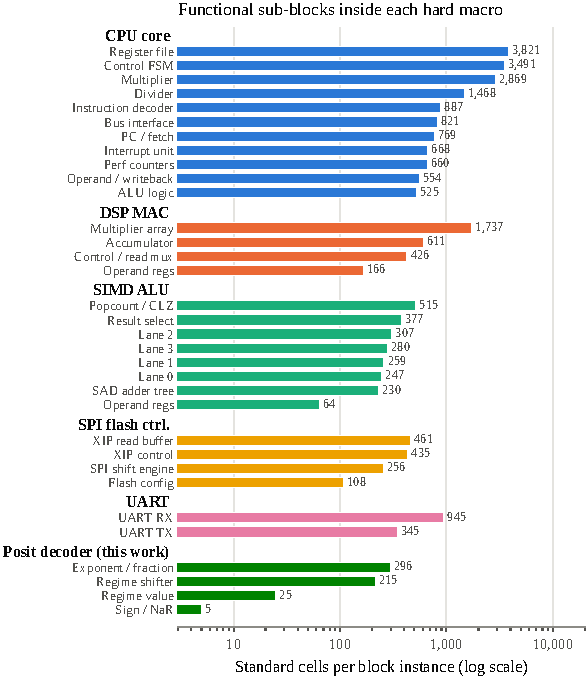
\includegraphics[width=\columnwidth]{fig02_subblock_cells.pdf}
\caption{Standard cells per functional sub-block in each hard macro. A netlist cone analysis assigns every logic cell to one sub-block.}
\label{fig:subblocks}
\end{figure}

\begin{figure*}[!t]
\centering
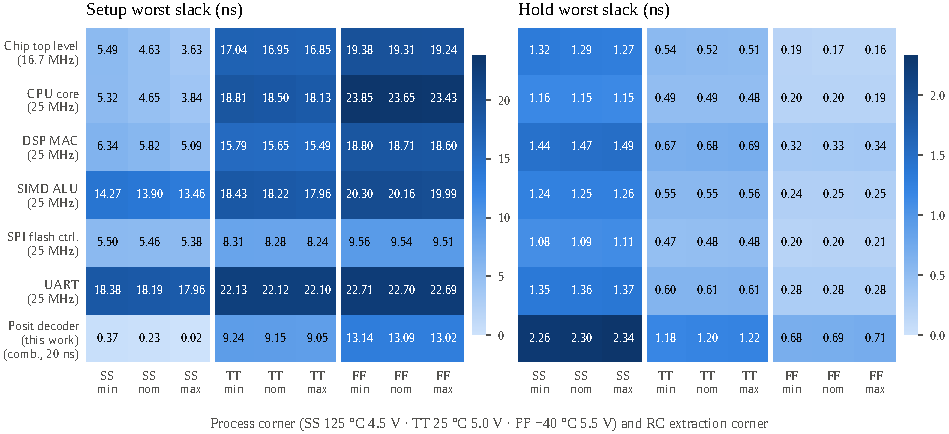
\includegraphics[width=\textwidth]{fig03_timing_heatmap.pdf}
\caption{Post-route worst setup and hold slack at nine process and RC corners. Every block meets timing at every corner. The posit decoder is combinational and meets a 20\,ns input-to-output constraint.}
\label{fig:timing}
\end{figure*}

\begin{figure*}[!t]
\centering
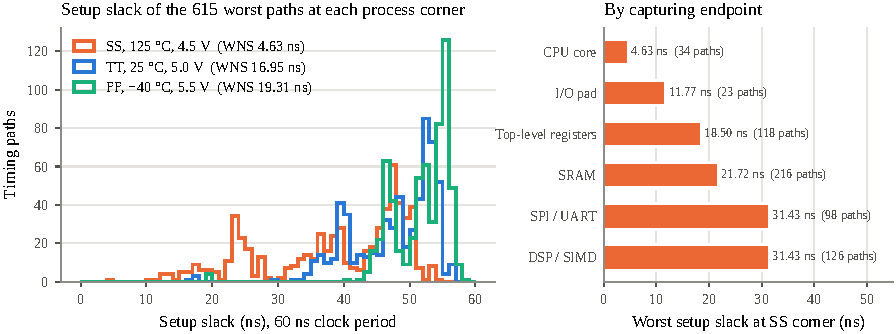
\includegraphics[width=\textwidth]{fig04_slack_distribution.pdf}
\caption{Setup slack of the worst top-level timing paths at a 60\,ns clock period. The right panel groups the slow-corner paths by capturing endpoint. The CPU bus paths set the worst slack.}
\label{fig:slack}
\end{figure*}

\begin{figure*}[!t]
\centering
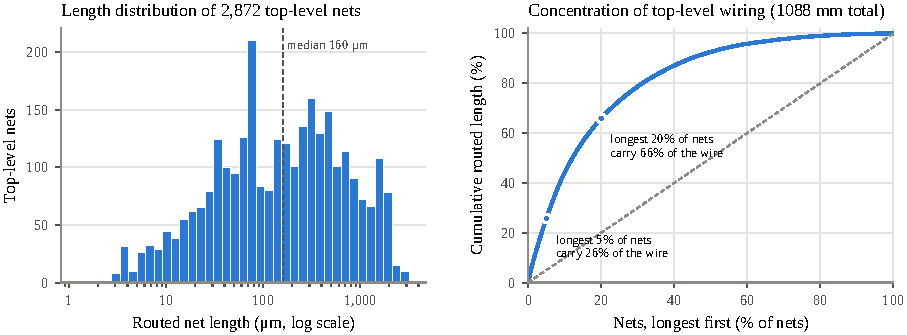
\includegraphics[width=\textwidth]{fig05_wirelength.pdf}
\caption{Routed length of the top-level nets. The longest 20\% of the nets carry 66\% of the top-level wire.}
\label{fig:wirelength}
\end{figure*}

\begin{figure}[!t]
\centering
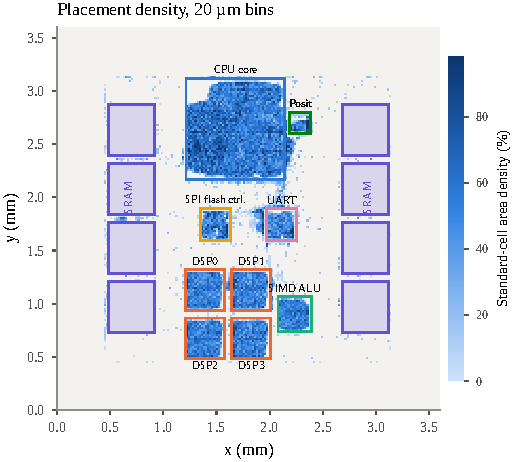
\includegraphics[width=\columnwidth]{fig06_density_map.pdf}
\caption{Standard-cell area density of the placed die in 20\,\textmu m bins. Outlines mark the hard macros; shaded boxes mark the foundry SRAM banks. The posit decoder sits beside the CPU core.}
\label{fig:density}
\end{figure}

\begin{figure}[!t]
\centering
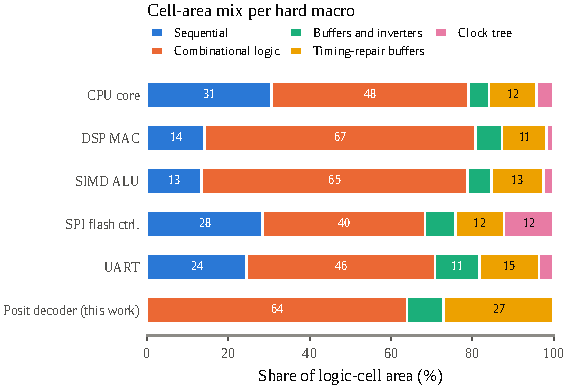
\includegraphics[width=\columnwidth]{fig07_cell_class_mix.pdf}
\caption{Logic-cell area by cell class for each hard macro. The posit decoder contains no sequential cells, as expected for a combinational datapath.}
\label{fig:classes}
\end{figure}

\begin{figure*}[!t]
\centering
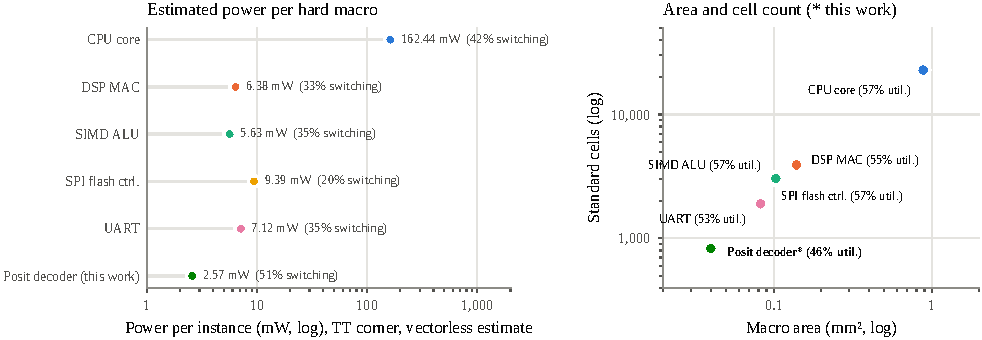
\includegraphics[width=\textwidth]{fig08_macro_power_area.pdf}
\caption{Estimated power, area and cell count of each hard macro. OpenSTA computes the power with default switching activity at the typical corner. The values support a relative comparison only.}
\label{fig:power}
\end{figure*}

\begin{figure*}[!t]
\centering
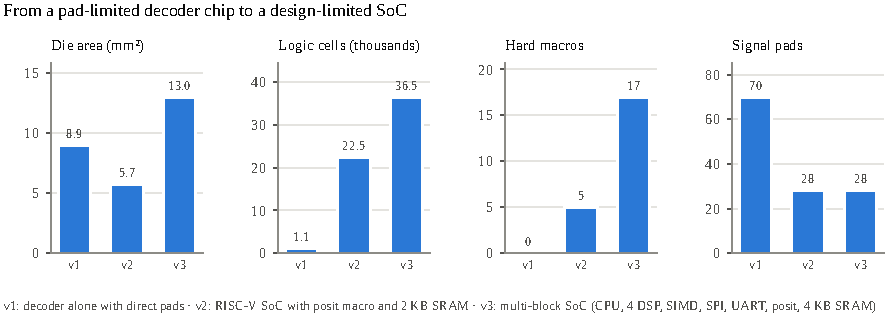
\includegraphics[width=\textwidth]{fig09_design_evolution.pdf}
\caption{Die area, logic cells, hard macros and signal pads of three design versions. The v1 chip is pad-limited; the v3 SoC is design-limited.}
\label{fig:evolution}
\end{figure*}

\begin{figure*}[!t]
\centering
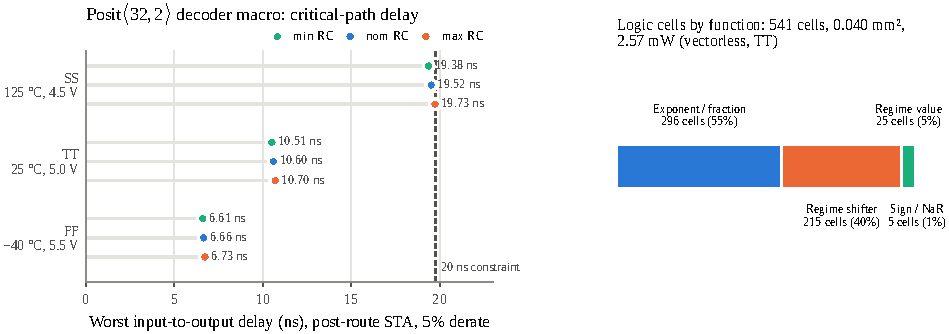
\includegraphics[width=\textwidth]{fig10_posit_decoder.pdf}
\caption{Proposed posit$\langle 32,2\rangle$ decoder macro. Left: post-route worst input-to-output delay at nine corners, including a 5\% timing derate. Right: logic cells grouped by function.}
\label{fig:posit}
\end{figure*}
